\chapter{Choix automatique du nombre de classe.}

\section{Algorithme 1 : Analyse des valeurs propres et le n-gap}

Dans le cas d'une classification idéale, la matrice laplacienne $L$ peut être mise sous la d'une matrice par bloc où tout les blocs non-diagonaux sont nuls.

\medskip

$
L = 
\begin{bmatrix}
   x^{(1)} &0 &\cdots &0 \\
   0 &x^{(2)} &\ddots &\vdots\\
   \vdots &\ddots &\ddots &0\\
   0 &\cdots &0 &x^{(n)}
\end{bmatrix}
$

\medskip

Cela traduit le fait que les blocs ou clusters sont homogènes et ne présentent pas de similitude entre eux. Cependant, vu comment la matrice L est construite, la valeur propre 0 va avoir une multiplicité égale au nombre de bloc.

\medskip

Une première méthode consiste donc à afficher les $n$ premières valeurs propres de L et de "compter" le nombre de fois que la valeur propre 0 apparait. Dans le cas des données simulées ci-dessous:

\medskip

\begin{figure}[H]
\centering
    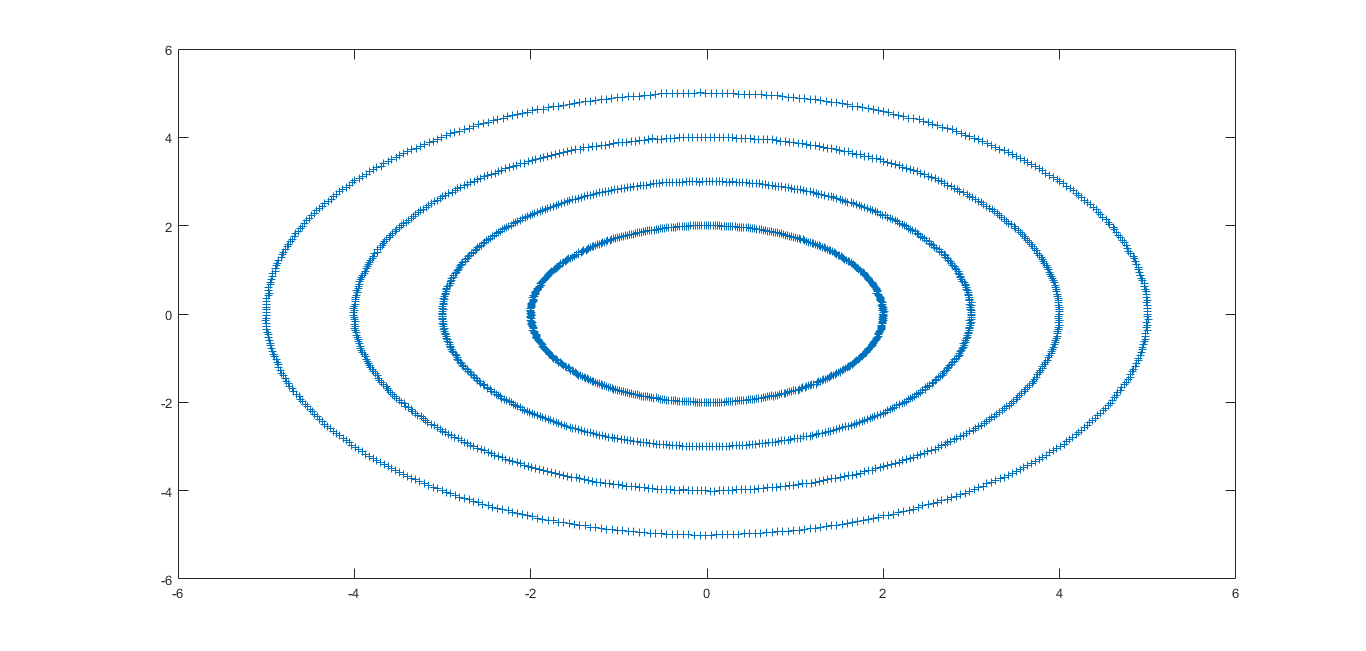
\includegraphics[scale=0.4,angle=0]{Images/testData.png}
    \caption{Exemple simple de données à classifier. Le nombre de classe est 4.}
    \label{fig:testData}
\end{figure} 

\medskip

Nous arrivons au valeurs propres suivantes:

\medskip

\begin{figure}[H]
\centering
    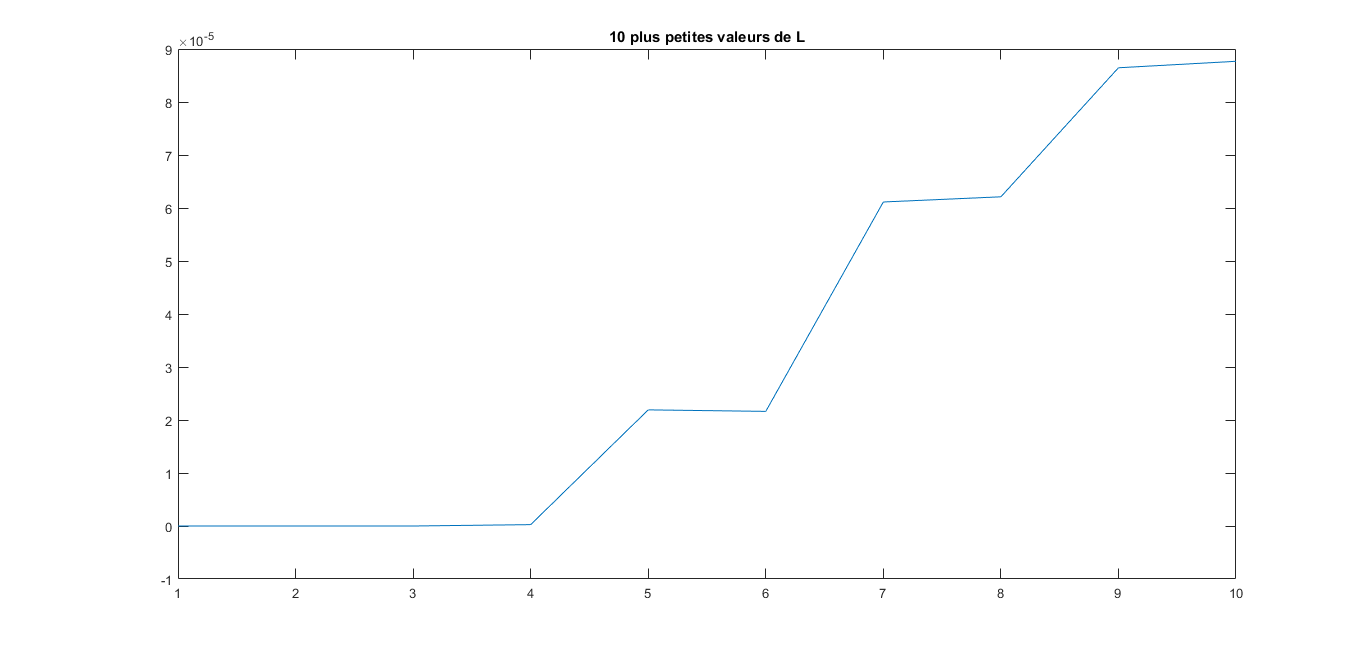
\includegraphics[scale=0.4,angle=0]{Images/Ngap.png}
    \caption{10 plus petites valeurs propres de L. On observe bien que on a un saut à partir de n=5. Le nombre optimal de classe est 4.}
    \label{fig:Ngap}
\end{figure} 

\medskip

Une autre méthode consiste à calculer la différence entre deux valeurs propres successives et voir à partir de quand un gap significatif se produit afin d'identifier le nombre de classe optimale. Néanmoins, ces deux méthodes sont hautement discutables de par leur manque de rigueur.


\section{Algorithme 2 : Minimisation par la norme de Frobenius}

Une autre méthode consiste à voir pour quel nombre de classe la similitude entre classe est la plus faible.
On définit la norme de Frobenius d'une matrice par la formule suivante:

\medskip
$
\|{L}\|_F = \sum_{i=1}^{N_i}  \sum_{j=1}^{N_j} |L_{ij}|
$
\medskip

L'idée va donc être de calculer le volume des blocs diagonaux et de calculer une fonction coût qui dépend du nombre de classe.

\begin{figure}[H]
\centering
    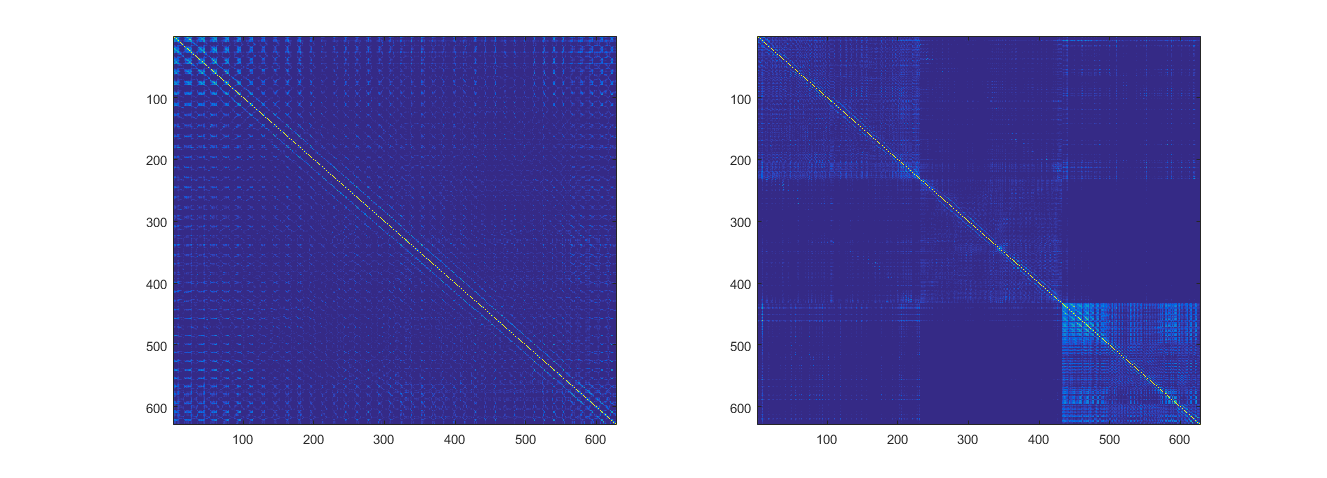
\includegraphics[scale=0.4,angle=0]{Images/L.png}
    \caption{Exemple de matrice laplacienne avant et après utilisation de l'algorithme de classification spectrale en trois classes et ré-agencement. On observe bien l'apparition de blocs.}
    \label{fig:L}
\end{figure} 

On définit donc le ratio de Frobenius entre deux blocs de la matrice L par:

\medskip

$
r_{ij} = \frac{ \|{L^{ij}}\|_F }{\| L^{ii} \|_F}
$

\medskip

On va donc regarder les valeurs de $r_{ij}$ et voir pour quel valeur de $n$ on atteint un minimum. Le but de cet algorithme va consister à trouver la valeur de $n$ qui va minimiser la fonction :

\medskip

$
\nu_k = \frac{2}{k(k-1)}\sum_{i=1 , j=i+1}^{k}(r_{ij})
$

\medskip

Il faut donc regarder pour plusieurs valeurs de n quel est le nombre de classe qui minimise cette fonction.

\section{Algorithme 2 : Minimisation par rotation}

Le dernier algorithme consiste à utiliser la même approche que précédemment mais 

\chapter{Application de ces algorithmes sur des données réelles}